%%%%%%%%%% POSSIBILITIES
\showCILC{true}{
	\begin{frame}{Overview}
		\begin{itemize}
			\item[-] Introduced by Gerbrandy and Groeneveld~\cite{Gerbrandy1997}
			\item[-] Used to represent \emphSlide{multi-agent information change}
			\item[-] Based on \emphSlide{\nwf\ sets}
			\item[-] Corresponds with a class of bisimilar Kripke structures~\cite{gerbrandy1999bisimulations}
		\end{itemize}
	\end{frame}
}

%%%%%%%%%% NWFSs
\showCILC{true}{
	\subsection*{\Nwf\ sets theory}
}

%\showCILC{true}{\begin{frame}{\Wf\ sets}
%		\begin{block}{\Wf\ set}
%			Let $E$ be a set, $E^\prime$ one of its elements, $E^{\prime\prime}$ any element of $E^\prime$, and so on. A descent is the sequence of steps from $E$ to $E^\prime$, $E^\prime$ to $E^{\prime\prime}$, etc.  A set is 
%			\alert{\wf}\ (or \emph{ordinary}) when it only gives rise to \emph{finite} descents.
%		\end{block}
%	
%	\vspace{-0.3cm}
%		\begin{figure}
%			{\scalebox{0.6}{

\tikzset{every picture/.style={line width=0.75pt}} %set default line width to 0.75pt        

\begin{tikzpicture}[x=0.75pt,y=0.75pt,yscale=-0.7,xscale=0.7]
%uncomment if require: \path (0,243); %set diagram left start at 0, and has height of 243

%Straight Lines [id:da42363008311855377] 
\draw    (126.5,47) ;
\draw [shift={(126.5,47)}, rotate = 0] [color={rgb, 255:red, 0; green, 0; blue, 0 }  ][fill={rgb, 255:red, 0; green, 0; blue, 0 }  ][line width=0.75]      (0, 0) circle [x radius= 3.35, y radius= 3.35]   ;

%Straight Lines [id:da9776475110732991] 
\draw    (196.5,47) -- (196.5,111) ;
\draw [shift={(196.5,111)}, rotate = 90] [color={rgb, 255:red, 0; green, 0; blue, 0 }  ][fill={rgb, 255:red, 0; green, 0; blue, 0 }  ][line width=0.75]      (0, 0) circle [x radius= 3.35, y radius= 3.35]   ;
\draw [shift={(196.5,47)}, rotate = 90] [color={rgb, 255:red, 0; green, 0; blue, 0 }  ][fill={rgb, 255:red, 0; green, 0; blue, 0 }  ][line width=0.75]      (0, 0) circle [x radius= 3.35, y radius= 3.35]   ;
%Straight Lines [id:da161306486001776] 
\draw    (300.5,47) -- (274.5,110) ;
\draw [shift={(274.5,110)}, rotate = 112.43] [color={rgb, 255:red, 0; green, 0; blue, 0 }  ][fill={rgb, 255:red, 0; green, 0; blue, 0 }  ][line width=0.75]      (0, 0) circle [x radius= 3.35, y radius= 3.35]   ;
\draw [shift={(300.5,47)}, rotate = 112.43] [color={rgb, 255:red, 0; green, 0; blue, 0 }  ][fill={rgb, 255:red, 0; green, 0; blue, 0 }  ][line width=0.75]      (0, 0) circle [x radius= 3.35, y radius= 3.35]   ;
%Straight Lines [id:da12831723727076116] 
\draw    (300.5,47) -- (323.5,110) ;
\draw [shift={(323.5,110)}, rotate = 69.94] [color={rgb, 255:red, 0; green, 0; blue, 0 }  ][fill={rgb, 255:red, 0; green, 0; blue, 0 }  ][line width=0.75]      (0, 0) circle [x radius= 3.35, y radius= 3.35]   ;
\draw [shift={(300.5,47)}, rotate = 69.94] [color={rgb, 255:red, 0; green, 0; blue, 0 }  ][fill={rgb, 255:red, 0; green, 0; blue, 0 }  ][line width=0.75]      (0, 0) circle [x radius= 3.35, y radius= 3.35]   ;
%Straight Lines [id:da5112115278285075] 
\draw    (323.5,110) -- (323.5,172) ;
\draw [shift={(323.5,172)}, rotate = 90] [color={rgb, 255:red, 0; green, 0; blue, 0 }  ][fill={rgb, 255:red, 0; green, 0; blue, 0 }  ][line width=0.75]      (0, 0) circle [x radius= 3.35, y radius= 3.35]   ;
\draw [shift={(323.5,110)}, rotate = 90] [color={rgb, 255:red, 0; green, 0; blue, 0 }  ][fill={rgb, 255:red, 0; green, 0; blue, 0 }  ][line width=0.75]      (0, 0) circle [x radius= 3.35, y radius= 3.35]   ;
%Straight Lines [id:da8536132167008245] 
\draw    (426.5,46) -- (400.5,109) ;
\draw [shift={(400.5,109)}, rotate = 112.43] [color={rgb, 255:red, 0; green, 0; blue, 0 }  ][fill={rgb, 255:red, 0; green, 0; blue, 0 }  ][line width=0.75]      (0, 0) circle [x radius= 3.35, y radius= 3.35]   ;
\draw [shift={(426.5,46)}, rotate = 112.43] [color={rgb, 255:red, 0; green, 0; blue, 0 }  ][fill={rgb, 255:red, 0; green, 0; blue, 0 }  ][line width=0.75]      (0, 0) circle [x radius= 3.35, y radius= 3.35]   ;
%Straight Lines [id:da7449065643500326] 
\draw    (426.5,46) -- (449.5,109) ;
\draw [shift={(449.5,109)}, rotate = 69.94] [color={rgb, 255:red, 0; green, 0; blue, 0 }  ][fill={rgb, 255:red, 0; green, 0; blue, 0 }  ][line width=0.75]      (0, 0) circle [x radius= 3.35, y radius= 3.35]   ;
\draw [shift={(426.5,46)}, rotate = 69.94] [color={rgb, 255:red, 0; green, 0; blue, 0 }  ][fill={rgb, 255:red, 0; green, 0; blue, 0 }  ][line width=0.75]      (0, 0) circle [x radius= 3.35, y radius= 3.35]   ;
%Straight Lines [id:da07257306396931185] 
\draw    (449.5,109) -- (449.5,171) ;
\draw [shift={(449.5,171)}, rotate = 90] [color={rgb, 255:red, 0; green, 0; blue, 0 }  ][fill={rgb, 255:red, 0; green, 0; blue, 0 }  ][line width=0.75]      (0, 0) circle [x radius= 3.35, y radius= 3.35]   ;
\draw [shift={(449.5,109)}, rotate = 90] [color={rgb, 255:red, 0; green, 0; blue, 0 }  ][fill={rgb, 255:red, 0; green, 0; blue, 0 }  ][line width=0.75]      (0, 0) circle [x radius= 3.35, y radius= 3.35]   ;
%Straight Lines [id:da021322635576809246] 
\draw    (426.5,46) -- (494.5,110) ;
\draw [shift={(494.5,110)}, rotate = 43.26] [color={rgb, 255:red, 0; green, 0; blue, 0 }  ][fill={rgb, 255:red, 0; green, 0; blue, 0 }  ][line width=0.75]      (0, 0) circle [x radius= 3.35, y radius= 3.35]   ;
\draw [shift={(426.5,46)}, rotate = 43.26] [color={rgb, 255:red, 0; green, 0; blue, 0 }  ][fill={rgb, 255:red, 0; green, 0; blue, 0 }  ][line width=0.75]      (0, 0) circle [x radius= 3.35, y radius= 3.35]   ;
%Straight Lines [id:da9755353003788908] 
\draw    (494.5,110) -- (468.5,173) ;
\draw [shift={(468.5,173)}, rotate = 112.43] [color={rgb, 255:red, 0; green, 0; blue, 0 }  ][fill={rgb, 255:red, 0; green, 0; blue, 0 }  ][line width=0.75]      (0, 0) circle [x radius= 3.35, y radius= 3.35]   ;
\draw [shift={(494.5,110)}, rotate = 112.43] [color={rgb, 255:red, 0; green, 0; blue, 0 }  ][fill={rgb, 255:red, 0; green, 0; blue, 0 }  ][line width=0.75]      (0, 0) circle [x radius= 3.35, y radius= 3.35]   ;
%Straight Lines [id:da12250203413215166] 
\draw    (494.5,110) -- (517.5,173) ;
\draw [shift={(517.5,173)}, rotate = 69.94] [color={rgb, 255:red, 0; green, 0; blue, 0 }  ][fill={rgb, 255:red, 0; green, 0; blue, 0 }  ][line width=0.75]      (0, 0) circle [x radius= 3.35, y radius= 3.35]   ;
\draw [shift={(494.5,110)}, rotate = 69.94] [color={rgb, 255:red, 0; green, 0; blue, 0 }  ][fill={rgb, 255:red, 0; green, 0; blue, 0 }  ][line width=0.75]      (0, 0) circle [x radius= 3.35, y radius= 3.35]   ;
%Straight Lines [id:da4220154805716767] 
\draw    (517.5,173) -- (517.5,235) ;
\draw [shift={(517.5,235)}, rotate = 90] [color={rgb, 255:red, 0; green, 0; blue, 0 }  ][fill={rgb, 255:red, 0; green, 0; blue, 0 }  ][line width=0.75]      (0, 0) circle [x radius= 3.35, y radius= 3.35]   ;
\draw [shift={(517.5,173)}, rotate = 90] [color={rgb, 255:red, 0; green, 0; blue, 0 }  ][fill={rgb, 255:red, 0; green, 0; blue, 0 }  ][line width=0.75]      (0, 0) circle [x radius= 3.35, y radius= 3.35]   ;
%Straight Lines [id:da34828451096237323] 
\draw    (438,77.5) -- (441.87,89.1) ;
\draw [shift={(442.5,91)}, rotate = 251.57] [fill={rgb, 255:red, 0; green, 0; blue, 0 }  ][line width=0.75]  [draw opacity=0] (8.93,-4.29) -- (0,0) -- (8.93,4.29) -- cycle    ;

%Straight Lines [id:da847083601142183] 
\draw    (413.5,77.5) -- (410.21,86.13) ;
\draw [shift={(409.5,88)}, rotate = 290.85] [fill={rgb, 255:red, 0; green, 0; blue, 0 }  ][line width=0.75]  [draw opacity=0] (8.93,-4.29) -- (0,0) -- (8.93,4.29) -- cycle    ;

%Straight Lines [id:da8305126214716252] 
\draw    (449.5,137) -- (449.5,145) ;
\draw [shift={(449.5,147)}, rotate = 270] [fill={rgb, 255:red, 0; green, 0; blue, 0 }  ][line width=0.75]  [draw opacity=0] (8.93,-4.29) -- (0,0) -- (8.93,4.29) -- cycle    ;

%Straight Lines [id:da0020619886975261625] 
\draw    (506,141.5) -- (509.77,151.14) ;
\draw [shift={(510.5,153)}, rotate = 248.63] [fill={rgb, 255:red, 0; green, 0; blue, 0 }  ][line width=0.75]  [draw opacity=0] (8.93,-4.29) -- (0,0) -- (8.93,4.29) -- cycle    ;

%Straight Lines [id:da8008262780720901] 
\draw    (517.5,204) -- (517.5,212) ;
\draw [shift={(517.5,214)}, rotate = 270] [fill={rgb, 255:red, 0; green, 0; blue, 0 }  ][line width=0.75]  [draw opacity=0] (8.93,-4.29) -- (0,0) -- (8.93,4.29) -- cycle    ;

%Straight Lines [id:da5166796275526594] 
\draw    (481.5,141.5) -- (477.3,151.17) ;
\draw [shift={(476.5,153)}, rotate = 293.5] [fill={rgb, 255:red, 0; green, 0; blue, 0 }  ][line width=0.75]  [draw opacity=0] (8.93,-4.29) -- (0,0) -- (8.93,4.29) -- cycle    ;

%Straight Lines [id:da2483045453323448] 
\draw    (460.5,78) -- (472.03,88.64) ;
\draw [shift={(473.5,90)}, rotate = 222.71] [fill={rgb, 255:red, 0; green, 0; blue, 0 }  ][line width=0.75]  [draw opacity=0] (8.93,-4.29) -- (0,0) -- (8.93,4.29) -- cycle    ;


%Straight Lines [id:da5301987015108148] 
\draw    (196.5,69) -- (196.5,77) ;
\draw [shift={(196.5,79)}, rotate = 270] [fill={rgb, 255:red, 0; green, 0; blue, 0 }  ][line width=0.75]  [draw opacity=0] (8.93,-4.29) -- (0,0) -- (8.93,4.29) -- cycle    ;

%Straight Lines [id:da9808201842892292] 
\draw    (287.5,78.5) -- (282.22,92.13) ;
\draw [shift={(281.5,94)}, rotate = 291.15999999999997] [fill={rgb, 255:red, 0; green, 0; blue, 0 }  ][line width=0.75]  [draw opacity=0] (8.93,-4.29) -- (0,0) -- (8.93,4.29) -- cycle    ;

%Straight Lines [id:da9287523922345057] 
\draw    (313,82.5) -- (316.82,93.12) ;
\draw [shift={(317.5,95)}, rotate = 250.2] [fill={rgb, 255:red, 0; green, 0; blue, 0 }  ][line width=0.75]  [draw opacity=0] (8.93,-4.29) -- (0,0) -- (8.93,4.29) -- cycle    ;

%Straight Lines [id:da02578212493217935] 
\draw    (323.5,141) -- (323.5,149) ;
\draw [shift={(323.5,151)}, rotate = 270] [fill={rgb, 255:red, 0; green, 0; blue, 0 }  ][line width=0.75]  [draw opacity=0] (8.93,-4.29) -- (0,0) -- (8.93,4.29) -- cycle    ;


% Text Node
\draw (130,22) node   {$0$};
% Text Node
\draw (197,22) node   {$1$};
% Text Node
\draw (300,22) node   {$2$};
% Text Node
\draw (427,22) node   {$3$};


\draw (60,22) node   {};
\draw (585,22) node   {};


\end{tikzpicture}

}\label{subfig-1:von_neu_ord}}
%			\hspace{1cm}
%			{
%				\scalebox{0.8}{\tikzset{every picture/.style={line width=0.75pt}} %set default line width to 0.75pt        

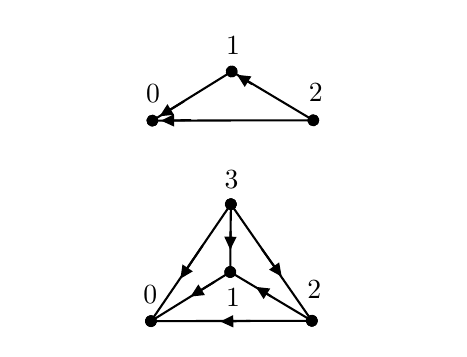
\begin{tikzpicture}[x=0.75pt,y=0.75pt,yscale=-0.7,xscale=0.7]\tikzset{every picture/.style={line width=0.75pt}}

%Straight Lines [id:da31341595090350494] 
\draw    (149.25,245.25) -- (38.5,245.5) ;
\draw [shift={(38.5,245.5)}, rotate = 179.87] [color={rgb, 255:red, 0; green, 0; blue, 0 }  ][fill={rgb, 255:red, 0; green, 0; blue, 0 }  ][line width=0.75]      (0, 0) circle [x radius= 3.35, y radius= 3.35]   ;
\draw [shift={(149.25,245.25)}, rotate = 179.87] [color={rgb, 255:red, 0; green, 0; blue, 0 }  ][fill={rgb, 255:red, 0; green, 0; blue, 0 }  ][line width=0.75]      (0, 0) circle [x radius= 3.35, y radius= 3.35]   ;
%Straight Lines [id:da9609296906616727] 
\draw    (106.88,245.38) -- (88.25,245.71) ;
\draw [shift={(86.25,245.75)}, rotate = 358.96000000000004] [fill={rgb, 255:red, 0; green, 0; blue, 0 }  ][line width=0.75]  [draw opacity=0] (8.93,-4.29) -- (0,0) -- (8.93,4.29) -- cycle    ;

%Straight Lines [id:da252345846123192] 
\draw    (93.5,165) -- (38.5,245.5) ;
\draw [shift={(38.5,245.5)}, rotate = 124.34] [color={rgb, 255:red, 0; green, 0; blue, 0 }  ][fill={rgb, 255:red, 0; green, 0; blue, 0 }  ][line width=0.75]      (0, 0) circle [x radius= 3.35, y radius= 3.35]   ;
\draw [shift={(93.5,165)}, rotate = 124.34] [color={rgb, 255:red, 0; green, 0; blue, 0 }  ][fill={rgb, 255:red, 0; green, 0; blue, 0 }  ][line width=0.75]      (0, 0) circle [x radius= 3.35, y radius= 3.35]   ;
%Straight Lines [id:da11171836378352906] 
\draw    (73.96,193.6) -- (59.88,214.61) ;
\draw [shift={(58.77,216.27)}, rotate = 303.83] [fill={rgb, 255:red, 0; green, 0; blue, 0 }  ][line width=0.75]  [draw opacity=0] (8.93,-4.29) -- (0,0) -- (8.93,4.29) -- cycle    ;

%Straight Lines [id:da9411846809932387] 
\draw    (149.25,245.25) -- (93.5,165) ;
\draw [shift={(93.5,165)}, rotate = 235.21] [color={rgb, 255:red, 0; green, 0; blue, 0 }  ][fill={rgb, 255:red, 0; green, 0; blue, 0 }  ][line width=0.75]      (0, 0) circle [x radius= 3.35, y radius= 3.35]   ;
\draw [shift={(149.25,245.25)}, rotate = 235.21] [color={rgb, 255:red, 0; green, 0; blue, 0 }  ][fill={rgb, 255:red, 0; green, 0; blue, 0 }  ][line width=0.75]      (0, 0) circle [x radius= 3.35, y radius= 3.35]   ;
%Straight Lines [id:da6467035917598132] 
\draw    (114.71,195.71) -- (127.31,213.19) ;
\draw [shift={(128.48,214.81)}, rotate = 234.21] [fill={rgb, 255:red, 0; green, 0; blue, 0 }  ][line width=0.75]  [draw opacity=0] (8.93,-4.29) -- (0,0) -- (8.93,4.29) -- cycle    ;

%Straight Lines [id:da05960945318721844] 
\draw    (93.5,165) -- (93.08,211.67) ;
\draw [shift={(93.08,211.67)}, rotate = 90.51] [color={rgb, 255:red, 0; green, 0; blue, 0 }  ][fill={rgb, 255:red, 0; green, 0; blue, 0 }  ][line width=0.75]      (0, 0) circle [x radius= 3.35, y radius= 3.35]   ;
\draw [shift={(93.5,165)}, rotate = 90.51] [color={rgb, 255:red, 0; green, 0; blue, 0 }  ][fill={rgb, 255:red, 0; green, 0; blue, 0 }  ][line width=0.75]      (0, 0) circle [x radius= 3.35, y radius= 3.35]   ;
%Straight Lines [id:da18779983245814547] 
\draw    (93.08,211.67) -- (38.5,245.5) ;
\draw [shift={(38.5,245.5)}, rotate = 148.21] [color={rgb, 255:red, 0; green, 0; blue, 0 }  ][fill={rgb, 255:red, 0; green, 0; blue, 0 }  ][line width=0.75]      (0, 0) circle [x radius= 3.35, y radius= 3.35]   ;
\draw [shift={(93.08,211.67)}, rotate = 148.21] [color={rgb, 255:red, 0; green, 0; blue, 0 }  ][fill={rgb, 255:red, 0; green, 0; blue, 0 }  ][line width=0.75]      (0, 0) circle [x radius= 3.35, y radius= 3.35]   ;
%Straight Lines [id:da9874513451972009] 
\draw    (93.08,211.67) -- (149.25,245.25) ;
\draw [shift={(149.25,245.25)}, rotate = 30.88] [color={rgb, 255:red, 0; green, 0; blue, 0 }  ][fill={rgb, 255:red, 0; green, 0; blue, 0 }  ][line width=0.75]      (0, 0) circle [x radius= 3.35, y radius= 3.35]   ;
\draw [shift={(93.08,211.67)}, rotate = 30.88] [color={rgb, 255:red, 0; green, 0; blue, 0 }  ][fill={rgb, 255:red, 0; green, 0; blue, 0 }  ][line width=0.75]      (0, 0) circle [x radius= 3.35, y radius= 3.35]   ;
%Straight Lines [id:da21738250880340737] 
\draw    (82.42,218.33) -- (67.49,227.53) ;
\draw [shift={(65.79,228.58)}, rotate = 328.34000000000003] [fill={rgb, 255:red, 0; green, 0; blue, 0 }  ][line width=0.75]  [draw opacity=0] (8.93,-4.29) -- (0,0) -- (8.93,4.29) -- cycle    ;

%Straight Lines [id:da502837847841804] 
\draw    (93.29,183.33) -- (93.13,194.32) ;
\draw [shift={(93.1,196.32)}, rotate = 270.83] [fill={rgb, 255:red, 0; green, 0; blue, 0 }  ][line width=0.75]  [draw opacity=0] (8.93,-4.29) -- (0,0) -- (8.93,4.29) -- cycle    ;

%Straight Lines [id:da38006772268977085] 
\draw    (121.17,228.46) -- (112.46,223) ;
\draw [shift={(110.76,221.94)}, rotate = 392.05] [fill={rgb, 255:red, 0; green, 0; blue, 0 }  ][line width=0.75]  [draw opacity=0] (8.93,-4.29) -- (0,0) -- (8.93,4.29) -- cycle    ;

%Straight Lines [id:da09733860617343582] 
\draw    (150.25,107.25) -- (39.5,107.5) ;
\draw [shift={(39.5,107.5)}, rotate = 179.87] [color={rgb, 255:red, 0; green, 0; blue, 0 }  ][fill={rgb, 255:red, 0; green, 0; blue, 0 }  ][line width=0.75]      (0, 0) circle [x radius= 3.35, y radius= 3.35]   ;
\draw [shift={(150.25,107.25)}, rotate = 179.87] [color={rgb, 255:red, 0; green, 0; blue, 0 }  ][fill={rgb, 255:red, 0; green, 0; blue, 0 }  ][line width=0.75]      (0, 0) circle [x radius= 3.35, y radius= 3.35]   ;
%Straight Lines [id:da9907229664589221] 
\draw    (66.13,107.13) -- (47.5,107.46) ;
\draw [shift={(45.5,107.5)}, rotate = 358.96000000000004] [fill={rgb, 255:red, 0; green, 0; blue, 0 }  ][line width=0.75]  [draw opacity=0] (8.93,-4.29) -- (0,0) -- (8.93,4.29) -- cycle    ;

%Straight Lines [id:da8984506786350759] 
\draw    (94.08,73.67) -- (39.5,107.5) ;
\draw [shift={(39.5,107.5)}, rotate = 148.21] [color={rgb, 255:red, 0; green, 0; blue, 0 }  ][fill={rgb, 255:red, 0; green, 0; blue, 0 }  ][line width=0.75]      (0, 0) circle [x radius= 3.35, y radius= 3.35]   ;
\draw [shift={(94.08,73.67)}, rotate = 148.21] [color={rgb, 255:red, 0; green, 0; blue, 0 }  ][fill={rgb, 255:red, 0; green, 0; blue, 0 }  ][line width=0.75]      (0, 0) circle [x radius= 3.35, y radius= 3.35]   ;
%Straight Lines [id:da13062093153249577] 
\draw    (94.08,73.67) -- (150.25,107.25) ;
\draw [shift={(150.25,107.25)}, rotate = 30.88] [color={rgb, 255:red, 0; green, 0; blue, 0 }  ][fill={rgb, 255:red, 0; green, 0; blue, 0 }  ][line width=0.75]      (0, 0) circle [x radius= 3.35, y radius= 3.35]   ;
\draw [shift={(94.08,73.67)}, rotate = 30.88] [color={rgb, 255:red, 0; green, 0; blue, 0 }  ][fill={rgb, 255:red, 0; green, 0; blue, 0 }  ][line width=0.75]      (0, 0) circle [x radius= 3.35, y radius= 3.35]   ;
%Straight Lines [id:da9384075142317254] 
\draw    (61.13,94.25) -- (46.2,103.45) ;
\draw [shift={(44.5,104.5)}, rotate = 328.34000000000003] [fill={rgb, 255:red, 0; green, 0; blue, 0 }  ][line width=0.75]  [draw opacity=0] (8.93,-4.29) -- (0,0) -- (8.93,4.29) -- cycle    ;

%Straight Lines [id:da2991130569955017] 
\draw    (108.17,82.46) -- (99.46,77) ;
\draw [shift={(97.76,75.94)}, rotate = 392.05] [fill={rgb, 255:red, 0; green, 0; blue, 0 }  ][line width=0.75]  [draw opacity=0] (8.93,-4.29) -- (0,0) -- (8.93,4.29) -- cycle    ;


% Text Node
\draw (94,148) node   {$3$};
% Text Node
\draw (152,88) node   {$2$};
% Text Node
\draw (95,56) node   {$1$};
% Text Node
\draw (151,224) node   {$2$};
% Text Node
\draw (95,229) node   {$1$};
% Text Node
\draw (38,227) node   {$0$};
% Text Node
\draw (40,89) node   {$0$};


\draw (-40,89) node   {};
\draw (230,56) node   {};

\end{tikzpicture}
}}
%			{\centering\\\onslide<2->{ von Neumann ordinals:\\
%					$0=\emptyset$;}
%				\onslide<3->{$1=\bra{\emptyset}$;}
%				\onslide<4->{$2=\bra{\emptyset, \bra{\emptyset}}$;}
%				\onslide<5->{$3=\bra{\emptyset,\bra{\emptyset},\bra{\emptyset,\bra{\emptyset}}}$}}
%		\end{figure}
%\end{frame}}
\showCILC{false}{
	\begin{frame}{\Wf\ sets}
		\begin{block}{\Wf\ set \cite{Aczel1989-ACZNS-2}}
			Let $E$ be a set, $E^\prime$ one of its elements, $E^{\prime\prime}$ any element of $E^\prime$, and so on. A \emphSlide{descent} is the sequence of steps from $E$ to $E^\prime$, $E^\prime$ to $E^{\prime\prime}$, etc.  A set is
			\emphSlide{\wf}\ (or \emphSlide{ordinary}) when it only gives rise to finite descents.
		\end{block}

		\vspace{-0.2cm}
		\begin{figure}
			{\scalebox{0.7}{

\tikzset{every picture/.style={line width=0.75pt}} %set default line width to 0.75pt        

\begin{tikzpicture}[x=0.75pt,y=0.75pt,yscale=-0.7,xscale=0.7]
%uncomment if require: \path (0,243); %set diagram left start at 0, and has height of 243

%Straight Lines [id:da42363008311855377] 
\draw    (126.5,47) ;
\draw [shift={(126.5,47)}, rotate = 0] [color={rgb, 255:red, 0; green, 0; blue, 0 }  ][fill={rgb, 255:red, 0; green, 0; blue, 0 }  ][line width=0.75]      (0, 0) circle [x radius= 3.35, y radius= 3.35]   ;

%Straight Lines [id:da9776475110732991] 
\draw    (196.5,47) -- (196.5,111) ;
\draw [shift={(196.5,111)}, rotate = 90] [color={rgb, 255:red, 0; green, 0; blue, 0 }  ][fill={rgb, 255:red, 0; green, 0; blue, 0 }  ][line width=0.75]      (0, 0) circle [x radius= 3.35, y radius= 3.35]   ;
\draw [shift={(196.5,47)}, rotate = 90] [color={rgb, 255:red, 0; green, 0; blue, 0 }  ][fill={rgb, 255:red, 0; green, 0; blue, 0 }  ][line width=0.75]      (0, 0) circle [x radius= 3.35, y radius= 3.35]   ;
%Straight Lines [id:da161306486001776] 
\draw    (300.5,47) -- (274.5,110) ;
\draw [shift={(274.5,110)}, rotate = 112.43] [color={rgb, 255:red, 0; green, 0; blue, 0 }  ][fill={rgb, 255:red, 0; green, 0; blue, 0 }  ][line width=0.75]      (0, 0) circle [x radius= 3.35, y radius= 3.35]   ;
\draw [shift={(300.5,47)}, rotate = 112.43] [color={rgb, 255:red, 0; green, 0; blue, 0 }  ][fill={rgb, 255:red, 0; green, 0; blue, 0 }  ][line width=0.75]      (0, 0) circle [x radius= 3.35, y radius= 3.35]   ;
%Straight Lines [id:da12831723727076116] 
\draw    (300.5,47) -- (323.5,110) ;
\draw [shift={(323.5,110)}, rotate = 69.94] [color={rgb, 255:red, 0; green, 0; blue, 0 }  ][fill={rgb, 255:red, 0; green, 0; blue, 0 }  ][line width=0.75]      (0, 0) circle [x radius= 3.35, y radius= 3.35]   ;
\draw [shift={(300.5,47)}, rotate = 69.94] [color={rgb, 255:red, 0; green, 0; blue, 0 }  ][fill={rgb, 255:red, 0; green, 0; blue, 0 }  ][line width=0.75]      (0, 0) circle [x radius= 3.35, y radius= 3.35]   ;
%Straight Lines [id:da5112115278285075] 
\draw    (323.5,110) -- (323.5,172) ;
\draw [shift={(323.5,172)}, rotate = 90] [color={rgb, 255:red, 0; green, 0; blue, 0 }  ][fill={rgb, 255:red, 0; green, 0; blue, 0 }  ][line width=0.75]      (0, 0) circle [x radius= 3.35, y radius= 3.35]   ;
\draw [shift={(323.5,110)}, rotate = 90] [color={rgb, 255:red, 0; green, 0; blue, 0 }  ][fill={rgb, 255:red, 0; green, 0; blue, 0 }  ][line width=0.75]      (0, 0) circle [x radius= 3.35, y radius= 3.35]   ;
%Straight Lines [id:da8536132167008245] 
\draw    (426.5,46) -- (400.5,109) ;
\draw [shift={(400.5,109)}, rotate = 112.43] [color={rgb, 255:red, 0; green, 0; blue, 0 }  ][fill={rgb, 255:red, 0; green, 0; blue, 0 }  ][line width=0.75]      (0, 0) circle [x radius= 3.35, y radius= 3.35]   ;
\draw [shift={(426.5,46)}, rotate = 112.43] [color={rgb, 255:red, 0; green, 0; blue, 0 }  ][fill={rgb, 255:red, 0; green, 0; blue, 0 }  ][line width=0.75]      (0, 0) circle [x radius= 3.35, y radius= 3.35]   ;
%Straight Lines [id:da7449065643500326] 
\draw    (426.5,46) -- (449.5,109) ;
\draw [shift={(449.5,109)}, rotate = 69.94] [color={rgb, 255:red, 0; green, 0; blue, 0 }  ][fill={rgb, 255:red, 0; green, 0; blue, 0 }  ][line width=0.75]      (0, 0) circle [x radius= 3.35, y radius= 3.35]   ;
\draw [shift={(426.5,46)}, rotate = 69.94] [color={rgb, 255:red, 0; green, 0; blue, 0 }  ][fill={rgb, 255:red, 0; green, 0; blue, 0 }  ][line width=0.75]      (0, 0) circle [x radius= 3.35, y radius= 3.35]   ;
%Straight Lines [id:da07257306396931185] 
\draw    (449.5,109) -- (449.5,171) ;
\draw [shift={(449.5,171)}, rotate = 90] [color={rgb, 255:red, 0; green, 0; blue, 0 }  ][fill={rgb, 255:red, 0; green, 0; blue, 0 }  ][line width=0.75]      (0, 0) circle [x radius= 3.35, y radius= 3.35]   ;
\draw [shift={(449.5,109)}, rotate = 90] [color={rgb, 255:red, 0; green, 0; blue, 0 }  ][fill={rgb, 255:red, 0; green, 0; blue, 0 }  ][line width=0.75]      (0, 0) circle [x radius= 3.35, y radius= 3.35]   ;
%Straight Lines [id:da021322635576809246] 
\draw    (426.5,46) -- (494.5,110) ;
\draw [shift={(494.5,110)}, rotate = 43.26] [color={rgb, 255:red, 0; green, 0; blue, 0 }  ][fill={rgb, 255:red, 0; green, 0; blue, 0 }  ][line width=0.75]      (0, 0) circle [x radius= 3.35, y radius= 3.35]   ;
\draw [shift={(426.5,46)}, rotate = 43.26] [color={rgb, 255:red, 0; green, 0; blue, 0 }  ][fill={rgb, 255:red, 0; green, 0; blue, 0 }  ][line width=0.75]      (0, 0) circle [x radius= 3.35, y radius= 3.35]   ;
%Straight Lines [id:da9755353003788908] 
\draw    (494.5,110) -- (468.5,173) ;
\draw [shift={(468.5,173)}, rotate = 112.43] [color={rgb, 255:red, 0; green, 0; blue, 0 }  ][fill={rgb, 255:red, 0; green, 0; blue, 0 }  ][line width=0.75]      (0, 0) circle [x radius= 3.35, y radius= 3.35]   ;
\draw [shift={(494.5,110)}, rotate = 112.43] [color={rgb, 255:red, 0; green, 0; blue, 0 }  ][fill={rgb, 255:red, 0; green, 0; blue, 0 }  ][line width=0.75]      (0, 0) circle [x radius= 3.35, y radius= 3.35]   ;
%Straight Lines [id:da12250203413215166] 
\draw    (494.5,110) -- (517.5,173) ;
\draw [shift={(517.5,173)}, rotate = 69.94] [color={rgb, 255:red, 0; green, 0; blue, 0 }  ][fill={rgb, 255:red, 0; green, 0; blue, 0 }  ][line width=0.75]      (0, 0) circle [x radius= 3.35, y radius= 3.35]   ;
\draw [shift={(494.5,110)}, rotate = 69.94] [color={rgb, 255:red, 0; green, 0; blue, 0 }  ][fill={rgb, 255:red, 0; green, 0; blue, 0 }  ][line width=0.75]      (0, 0) circle [x radius= 3.35, y radius= 3.35]   ;
%Straight Lines [id:da4220154805716767] 
\draw    (517.5,173) -- (517.5,235) ;
\draw [shift={(517.5,235)}, rotate = 90] [color={rgb, 255:red, 0; green, 0; blue, 0 }  ][fill={rgb, 255:red, 0; green, 0; blue, 0 }  ][line width=0.75]      (0, 0) circle [x radius= 3.35, y radius= 3.35]   ;
\draw [shift={(517.5,173)}, rotate = 90] [color={rgb, 255:red, 0; green, 0; blue, 0 }  ][fill={rgb, 255:red, 0; green, 0; blue, 0 }  ][line width=0.75]      (0, 0) circle [x radius= 3.35, y radius= 3.35]   ;
%Straight Lines [id:da34828451096237323] 
\draw    (438,77.5) -- (441.87,89.1) ;
\draw [shift={(442.5,91)}, rotate = 251.57] [fill={rgb, 255:red, 0; green, 0; blue, 0 }  ][line width=0.75]  [draw opacity=0] (8.93,-4.29) -- (0,0) -- (8.93,4.29) -- cycle    ;

%Straight Lines [id:da847083601142183] 
\draw    (413.5,77.5) -- (410.21,86.13) ;
\draw [shift={(409.5,88)}, rotate = 290.85] [fill={rgb, 255:red, 0; green, 0; blue, 0 }  ][line width=0.75]  [draw opacity=0] (8.93,-4.29) -- (0,0) -- (8.93,4.29) -- cycle    ;

%Straight Lines [id:da8305126214716252] 
\draw    (449.5,137) -- (449.5,145) ;
\draw [shift={(449.5,147)}, rotate = 270] [fill={rgb, 255:red, 0; green, 0; blue, 0 }  ][line width=0.75]  [draw opacity=0] (8.93,-4.29) -- (0,0) -- (8.93,4.29) -- cycle    ;

%Straight Lines [id:da0020619886975261625] 
\draw    (506,141.5) -- (509.77,151.14) ;
\draw [shift={(510.5,153)}, rotate = 248.63] [fill={rgb, 255:red, 0; green, 0; blue, 0 }  ][line width=0.75]  [draw opacity=0] (8.93,-4.29) -- (0,0) -- (8.93,4.29) -- cycle    ;

%Straight Lines [id:da8008262780720901] 
\draw    (517.5,204) -- (517.5,212) ;
\draw [shift={(517.5,214)}, rotate = 270] [fill={rgb, 255:red, 0; green, 0; blue, 0 }  ][line width=0.75]  [draw opacity=0] (8.93,-4.29) -- (0,0) -- (8.93,4.29) -- cycle    ;

%Straight Lines [id:da5166796275526594] 
\draw    (481.5,141.5) -- (477.3,151.17) ;
\draw [shift={(476.5,153)}, rotate = 293.5] [fill={rgb, 255:red, 0; green, 0; blue, 0 }  ][line width=0.75]  [draw opacity=0] (8.93,-4.29) -- (0,0) -- (8.93,4.29) -- cycle    ;

%Straight Lines [id:da2483045453323448] 
\draw    (460.5,78) -- (472.03,88.64) ;
\draw [shift={(473.5,90)}, rotate = 222.71] [fill={rgb, 255:red, 0; green, 0; blue, 0 }  ][line width=0.75]  [draw opacity=0] (8.93,-4.29) -- (0,0) -- (8.93,4.29) -- cycle    ;


%Straight Lines [id:da5301987015108148] 
\draw    (196.5,69) -- (196.5,77) ;
\draw [shift={(196.5,79)}, rotate = 270] [fill={rgb, 255:red, 0; green, 0; blue, 0 }  ][line width=0.75]  [draw opacity=0] (8.93,-4.29) -- (0,0) -- (8.93,4.29) -- cycle    ;

%Straight Lines [id:da9808201842892292] 
\draw    (287.5,78.5) -- (282.22,92.13) ;
\draw [shift={(281.5,94)}, rotate = 291.15999999999997] [fill={rgb, 255:red, 0; green, 0; blue, 0 }  ][line width=0.75]  [draw opacity=0] (8.93,-4.29) -- (0,0) -- (8.93,4.29) -- cycle    ;

%Straight Lines [id:da9287523922345057] 
\draw    (313,82.5) -- (316.82,93.12) ;
\draw [shift={(317.5,95)}, rotate = 250.2] [fill={rgb, 255:red, 0; green, 0; blue, 0 }  ][line width=0.75]  [draw opacity=0] (8.93,-4.29) -- (0,0) -- (8.93,4.29) -- cycle    ;

%Straight Lines [id:da02578212493217935] 
\draw    (323.5,141) -- (323.5,149) ;
\draw [shift={(323.5,151)}, rotate = 270] [fill={rgb, 255:red, 0; green, 0; blue, 0 }  ][line width=0.75]  [draw opacity=0] (8.93,-4.29) -- (0,0) -- (8.93,4.29) -- cycle    ;


% Text Node
\draw (130,22) node   {$0$};
% Text Node
\draw (197,22) node   {$1$};
% Text Node
\draw (300,22) node   {$2$};
% Text Node
\draw (427,22) node   {$3$};


\draw (60,22) node   {};
\draw (585,22) node   {};


\end{tikzpicture}

}\label{subfig-1:von_neu_ord}}
			\hfill
			{\scalebox{1}{\tikzset{every picture/.style={line width=0.75pt}} %set default line width to 0.75pt        

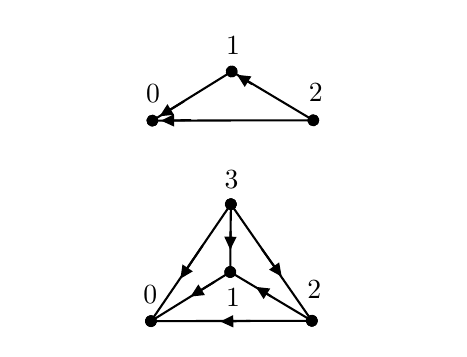
\begin{tikzpicture}[x=0.75pt,y=0.75pt,yscale=-0.7,xscale=0.7]\tikzset{every picture/.style={line width=0.75pt}}

%Straight Lines [id:da31341595090350494] 
\draw    (149.25,245.25) -- (38.5,245.5) ;
\draw [shift={(38.5,245.5)}, rotate = 179.87] [color={rgb, 255:red, 0; green, 0; blue, 0 }  ][fill={rgb, 255:red, 0; green, 0; blue, 0 }  ][line width=0.75]      (0, 0) circle [x radius= 3.35, y radius= 3.35]   ;
\draw [shift={(149.25,245.25)}, rotate = 179.87] [color={rgb, 255:red, 0; green, 0; blue, 0 }  ][fill={rgb, 255:red, 0; green, 0; blue, 0 }  ][line width=0.75]      (0, 0) circle [x radius= 3.35, y radius= 3.35]   ;
%Straight Lines [id:da9609296906616727] 
\draw    (106.88,245.38) -- (88.25,245.71) ;
\draw [shift={(86.25,245.75)}, rotate = 358.96000000000004] [fill={rgb, 255:red, 0; green, 0; blue, 0 }  ][line width=0.75]  [draw opacity=0] (8.93,-4.29) -- (0,0) -- (8.93,4.29) -- cycle    ;

%Straight Lines [id:da252345846123192] 
\draw    (93.5,165) -- (38.5,245.5) ;
\draw [shift={(38.5,245.5)}, rotate = 124.34] [color={rgb, 255:red, 0; green, 0; blue, 0 }  ][fill={rgb, 255:red, 0; green, 0; blue, 0 }  ][line width=0.75]      (0, 0) circle [x radius= 3.35, y radius= 3.35]   ;
\draw [shift={(93.5,165)}, rotate = 124.34] [color={rgb, 255:red, 0; green, 0; blue, 0 }  ][fill={rgb, 255:red, 0; green, 0; blue, 0 }  ][line width=0.75]      (0, 0) circle [x radius= 3.35, y radius= 3.35]   ;
%Straight Lines [id:da11171836378352906] 
\draw    (73.96,193.6) -- (59.88,214.61) ;
\draw [shift={(58.77,216.27)}, rotate = 303.83] [fill={rgb, 255:red, 0; green, 0; blue, 0 }  ][line width=0.75]  [draw opacity=0] (8.93,-4.29) -- (0,0) -- (8.93,4.29) -- cycle    ;

%Straight Lines [id:da9411846809932387] 
\draw    (149.25,245.25) -- (93.5,165) ;
\draw [shift={(93.5,165)}, rotate = 235.21] [color={rgb, 255:red, 0; green, 0; blue, 0 }  ][fill={rgb, 255:red, 0; green, 0; blue, 0 }  ][line width=0.75]      (0, 0) circle [x radius= 3.35, y radius= 3.35]   ;
\draw [shift={(149.25,245.25)}, rotate = 235.21] [color={rgb, 255:red, 0; green, 0; blue, 0 }  ][fill={rgb, 255:red, 0; green, 0; blue, 0 }  ][line width=0.75]      (0, 0) circle [x radius= 3.35, y radius= 3.35]   ;
%Straight Lines [id:da6467035917598132] 
\draw    (114.71,195.71) -- (127.31,213.19) ;
\draw [shift={(128.48,214.81)}, rotate = 234.21] [fill={rgb, 255:red, 0; green, 0; blue, 0 }  ][line width=0.75]  [draw opacity=0] (8.93,-4.29) -- (0,0) -- (8.93,4.29) -- cycle    ;

%Straight Lines [id:da05960945318721844] 
\draw    (93.5,165) -- (93.08,211.67) ;
\draw [shift={(93.08,211.67)}, rotate = 90.51] [color={rgb, 255:red, 0; green, 0; blue, 0 }  ][fill={rgb, 255:red, 0; green, 0; blue, 0 }  ][line width=0.75]      (0, 0) circle [x radius= 3.35, y radius= 3.35]   ;
\draw [shift={(93.5,165)}, rotate = 90.51] [color={rgb, 255:red, 0; green, 0; blue, 0 }  ][fill={rgb, 255:red, 0; green, 0; blue, 0 }  ][line width=0.75]      (0, 0) circle [x radius= 3.35, y radius= 3.35]   ;
%Straight Lines [id:da18779983245814547] 
\draw    (93.08,211.67) -- (38.5,245.5) ;
\draw [shift={(38.5,245.5)}, rotate = 148.21] [color={rgb, 255:red, 0; green, 0; blue, 0 }  ][fill={rgb, 255:red, 0; green, 0; blue, 0 }  ][line width=0.75]      (0, 0) circle [x radius= 3.35, y radius= 3.35]   ;
\draw [shift={(93.08,211.67)}, rotate = 148.21] [color={rgb, 255:red, 0; green, 0; blue, 0 }  ][fill={rgb, 255:red, 0; green, 0; blue, 0 }  ][line width=0.75]      (0, 0) circle [x radius= 3.35, y radius= 3.35]   ;
%Straight Lines [id:da9874513451972009] 
\draw    (93.08,211.67) -- (149.25,245.25) ;
\draw [shift={(149.25,245.25)}, rotate = 30.88] [color={rgb, 255:red, 0; green, 0; blue, 0 }  ][fill={rgb, 255:red, 0; green, 0; blue, 0 }  ][line width=0.75]      (0, 0) circle [x radius= 3.35, y radius= 3.35]   ;
\draw [shift={(93.08,211.67)}, rotate = 30.88] [color={rgb, 255:red, 0; green, 0; blue, 0 }  ][fill={rgb, 255:red, 0; green, 0; blue, 0 }  ][line width=0.75]      (0, 0) circle [x radius= 3.35, y radius= 3.35]   ;
%Straight Lines [id:da21738250880340737] 
\draw    (82.42,218.33) -- (67.49,227.53) ;
\draw [shift={(65.79,228.58)}, rotate = 328.34000000000003] [fill={rgb, 255:red, 0; green, 0; blue, 0 }  ][line width=0.75]  [draw opacity=0] (8.93,-4.29) -- (0,0) -- (8.93,4.29) -- cycle    ;

%Straight Lines [id:da502837847841804] 
\draw    (93.29,183.33) -- (93.13,194.32) ;
\draw [shift={(93.1,196.32)}, rotate = 270.83] [fill={rgb, 255:red, 0; green, 0; blue, 0 }  ][line width=0.75]  [draw opacity=0] (8.93,-4.29) -- (0,0) -- (8.93,4.29) -- cycle    ;

%Straight Lines [id:da38006772268977085] 
\draw    (121.17,228.46) -- (112.46,223) ;
\draw [shift={(110.76,221.94)}, rotate = 392.05] [fill={rgb, 255:red, 0; green, 0; blue, 0 }  ][line width=0.75]  [draw opacity=0] (8.93,-4.29) -- (0,0) -- (8.93,4.29) -- cycle    ;

%Straight Lines [id:da09733860617343582] 
\draw    (150.25,107.25) -- (39.5,107.5) ;
\draw [shift={(39.5,107.5)}, rotate = 179.87] [color={rgb, 255:red, 0; green, 0; blue, 0 }  ][fill={rgb, 255:red, 0; green, 0; blue, 0 }  ][line width=0.75]      (0, 0) circle [x radius= 3.35, y radius= 3.35]   ;
\draw [shift={(150.25,107.25)}, rotate = 179.87] [color={rgb, 255:red, 0; green, 0; blue, 0 }  ][fill={rgb, 255:red, 0; green, 0; blue, 0 }  ][line width=0.75]      (0, 0) circle [x radius= 3.35, y radius= 3.35]   ;
%Straight Lines [id:da9907229664589221] 
\draw    (66.13,107.13) -- (47.5,107.46) ;
\draw [shift={(45.5,107.5)}, rotate = 358.96000000000004] [fill={rgb, 255:red, 0; green, 0; blue, 0 }  ][line width=0.75]  [draw opacity=0] (8.93,-4.29) -- (0,0) -- (8.93,4.29) -- cycle    ;

%Straight Lines [id:da8984506786350759] 
\draw    (94.08,73.67) -- (39.5,107.5) ;
\draw [shift={(39.5,107.5)}, rotate = 148.21] [color={rgb, 255:red, 0; green, 0; blue, 0 }  ][fill={rgb, 255:red, 0; green, 0; blue, 0 }  ][line width=0.75]      (0, 0) circle [x radius= 3.35, y radius= 3.35]   ;
\draw [shift={(94.08,73.67)}, rotate = 148.21] [color={rgb, 255:red, 0; green, 0; blue, 0 }  ][fill={rgb, 255:red, 0; green, 0; blue, 0 }  ][line width=0.75]      (0, 0) circle [x radius= 3.35, y radius= 3.35]   ;
%Straight Lines [id:da13062093153249577] 
\draw    (94.08,73.67) -- (150.25,107.25) ;
\draw [shift={(150.25,107.25)}, rotate = 30.88] [color={rgb, 255:red, 0; green, 0; blue, 0 }  ][fill={rgb, 255:red, 0; green, 0; blue, 0 }  ][line width=0.75]      (0, 0) circle [x radius= 3.35, y radius= 3.35]   ;
\draw [shift={(94.08,73.67)}, rotate = 30.88] [color={rgb, 255:red, 0; green, 0; blue, 0 }  ][fill={rgb, 255:red, 0; green, 0; blue, 0 }  ][line width=0.75]      (0, 0) circle [x radius= 3.35, y radius= 3.35]   ;
%Straight Lines [id:da9384075142317254] 
\draw    (61.13,94.25) -- (46.2,103.45) ;
\draw [shift={(44.5,104.5)}, rotate = 328.34000000000003] [fill={rgb, 255:red, 0; green, 0; blue, 0 }  ][line width=0.75]  [draw opacity=0] (8.93,-4.29) -- (0,0) -- (8.93,4.29) -- cycle    ;

%Straight Lines [id:da2991130569955017] 
\draw    (108.17,82.46) -- (99.46,77) ;
\draw [shift={(97.76,75.94)}, rotate = 392.05] [fill={rgb, 255:red, 0; green, 0; blue, 0 }  ][line width=0.75]  [draw opacity=0] (8.93,-4.29) -- (0,0) -- (8.93,4.29) -- cycle    ;


% Text Node
\draw (94,148) node   {$3$};
% Text Node
\draw (152,88) node   {$2$};
% Text Node
\draw (95,56) node   {$1$};
% Text Node
\draw (151,224) node   {$2$};
% Text Node
\draw (95,229) node   {$1$};
% Text Node
\draw (38,227) node   {$0$};
% Text Node
\draw (40,89) node   {$0$};


\draw (-40,89) node   {};
\draw (230,56) node   {};

\end{tikzpicture}
}}
		\end{figure}
		\centering von Neumann ordinals:\\
		$0=\emptyset$;
		$1=\bra{\emptyset}$;
		$2=\bra{\emptyset, \bra{\emptyset}}$;
		$3=\bra{\emptyset,\bra{\emptyset},\bra{\emptyset,\bra{\emptyset}}}$
	\end{frame}
}

\showCILC{true}{
	\begin{frame}{\Nwf\ sets}
		\begin{block}{\Nwf\ set~\cite{Aczel1989-ACZNS-2}}
			A set is \emphSlide{\nwf}\ (or \emphSlide{extraordinary}) when among its descents there are some which are infinite.
		\end{block}
		\centering
		\begin{figure}
			{\scalebox{0.6}{\input{img/omega}}}
			\hfill
			{\scalebox{1.2}{

\tikzset{every picture/.style={line width=0.75pt}} %set default line width to 0.75pt        

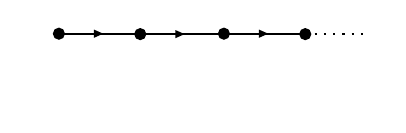
\begin{tikzpicture}[x=0.75pt,y=0.75pt,yscale=-1,xscale=1]
%uncomment if require: \path (0,300); %set diagram left start at 0, and has height of 300

%Straight Lines [id:da6276790682079358] 
\draw    (100.6,110) -- (140.85,110) ;


%Flowchart: Connector [id:dp10712755168097865] 
\draw  [fill={rgb, 255:red, 0; green, 0; blue, 0 }  ,fill opacity=1 ] (103,110) .. controls (103,111.33) and (101.93,112.4) .. (100.6,112.4) .. controls (99.27,112.4) and (98.2,111.33) .. (98.2,110) .. controls (98.2,108.67) and (99.27,107.6) .. (100.6,107.6) .. controls (101.93,107.6) and (103,108.67) .. (103,110) -- cycle ;
%Straight Lines [id:da8191358904406301] 
\draw    (139.8,110.2) -- (180.05,110.2) ;


%Flowchart: Connector [id:dp9628511983929124] 
\draw  [fill={rgb, 255:red, 0; green, 0; blue, 0 }  ,fill opacity=1 ] (142.2,110.2) .. controls (142.2,111.53) and (141.13,112.6) .. (139.8,112.6) .. controls (138.47,112.6) and (137.4,111.53) .. (137.4,110.2) .. controls (137.4,108.87) and (138.47,107.8) .. (139.8,107.8) .. controls (141.13,107.8) and (142.2,108.87) .. (142.2,110.2) -- cycle ;
%Shape: Triangle [id:dp18185199166706778] 
\draw  [fill={rgb, 255:red, 0; green, 0; blue, 0 }  ,fill opacity=1 ] (120.72,110) -- (118,111.21) -- (118,108.79) -- cycle ;
%Shape: Triangle [id:dp11767706980455106] 
\draw  [color={rgb, 255:red, 0; green, 0; blue, 0 }  ,draw opacity=1 ][fill={rgb, 255:red, 0; green, 0; blue, 0 }  ,fill opacity=1 ] (159.92,110.2) -- (157.2,111.41) -- (157.2,108.99) -- cycle ;
%Straight Lines [id:da6334935852876922] 
\draw    (180.1,110) -- (220.35,110) ;


%Flowchart: Connector [id:dp022374442404981654] 
\draw  [fill={rgb, 255:red, 0; green, 0; blue, 0 }  ,fill opacity=1 ] (182.5,110) .. controls (182.5,111.33) and (181.43,112.4) .. (180.1,112.4) .. controls (178.77,112.4) and (177.7,111.33) .. (177.7,110) .. controls (177.7,108.67) and (178.77,107.6) .. (180.1,107.6) .. controls (181.43,107.6) and (182.5,108.67) .. (182.5,110) -- cycle ;
%Flowchart: Connector [id:dp8113410302855639] 
\draw  [fill={rgb, 255:red, 0; green, 0; blue, 0 }  ,fill opacity=1 ] (221.7,110.2) .. controls (221.7,111.53) and (220.63,112.6) .. (219.3,112.6) .. controls (217.97,112.6) and (216.9,111.53) .. (216.9,110.2) .. controls (216.9,108.87) and (217.97,107.8) .. (219.3,107.8) .. controls (220.63,107.8) and (221.7,108.87) .. (221.7,110.2) -- cycle ;
%Shape: Triangle [id:dp5972516863295354] 
\draw  [fill={rgb, 255:red, 0; green, 0; blue, 0 }  ,fill opacity=1 ] (200.22,110) -- (197.5,111.21) -- (197.5,108.79) -- cycle ;
%Straight Lines [id:da9015443131541547] 
\draw  [dash pattern={on 0.84pt off 2.51pt}]  (219.3,110.2) -- (250.15,110.2) ;

\draw (250,140) node   {};
\draw (90,140) node   {};


\end{tikzpicture}

}}
			\\
			The \nwf\ set $\Omega = \{\Omega\}$
		\end{figure}
	\end{frame}
}

\showCILC{false}{
	\begin{frame}{Consequences}

		\begin{columns}[T] % align columns
			\begin{column}{.48\textwidth}
				{\color{black}\rule{\linewidth}{4pt}
					\Wf\ set Theory}
				\begin{center}
					\emph{Only \wf\ graphs have decorations \textbf{(FA)}\tikzmark{conseqa}}\\
					$\mathbf{\downarrow}$\\
					\emph{Each \wf\ graph is a picture of exactly one set\tikzmark{conseqc}}
				\end{center}

			\end{column}%
			\hfill%
			\onslide<2->{\begin{column}{.48\textwidth}
					{\emphColorSlide{\rule{\linewidth}{4pt}
							\Nwf\ set Theory}}
					\begin{center}
						{\color{ForestGreen!80!white}\emph{Every graph has a decoration \tikzmark{conseqb}\textbf{(AFA)}}\\
							\textbf{$\downarrow$}\\
							\emph{Every graph is a picture of \tikzmark{conseqd}exactly one set}}
					\end{center}
				\end{column}}%
		\end{columns}
		\onslide<2->{\begin{tikzpicture}[overlay,remember picture]
				\draw[very thick, -Stealth, ForestGreen] ($({pic cs:conseqc})+(1.5ex,9.5ex)$) to ($({pic cs:conseqd})+(-6ex,9.5ex)$);
				\draw[very thick, -Stealth, ForestGreen] ($({pic cs:conseqc})+(1.5ex,1.5ex)$) to ($({pic cs:conseqd})+(-6ex,1.5ex)$);
			\end{tikzpicture}
		}

	\end{frame}
}
\subsection*{}
%	\showCILC{true}{\begin{frame}{From \PosS\ to Kripke Structures}
%		A \nwf\ set can be expressed as a \emph{system of equations}
%		\begin{center}
%			\begin{figure}
%			{\scalebox{0.6}{

\tikzset{every picture/.style={line width=0.75pt}} %set default line width to 0.75pt        

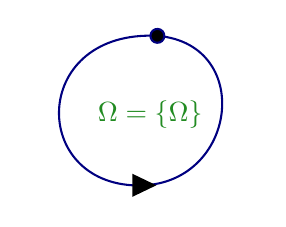
\begin{tikzpicture}[x=0.75pt,y=0.75pt,yscale=-1,xscale=1]
%uncomment if require: \path (0,243); %set diagram left start at 0, and has height of 243

%Curve Lines [id:da9361500626799328] 
\draw [NavyBlue]   (103.5,82) .. controls (151.5,86) and (141.5,157) .. (91.5,154) .. controls (41.5,151) and (43.5,79) .. (103.5,82) -- cycle ;
\draw [shift={(103.5,82)}, rotate = 2.86] [color=NavyBlue][fill={rgb, 255:red, 0; green, 0; blue, 0 }  ][line width=0.75]      (0, 0) circle [x radius= 3.35, y radius= 3.35]   ;

%Straight Lines [id:da3323560662413527] 
\draw [line width=1.5]    (103,154) ;
\draw [shift={(103,154)}, rotate = 180, color=NavyBlue] [fill={rgb, 255:red, 0; green, 0; blue, 0 }  ][line width=1.5]  [draw opacity=0] (11.61,-5.58) -- (0,0) -- (11.61,5.58) -- cycle    ;
\draw[color=ForestGreen] (100,120) node   {$\Omega=\{\Omega\}$};


\end{tikzpicture}

}}
%			\end{figure}
%		\end{center}
%		\vspace{-0.5cm}
%		\begin{center}
%			\textbf{Graphs} and \textbf{system of equations} are representation for \nwf\ set.\\
%			\vspace{0.2cm}
%			\onslide<2->{
%			Each graph has a \emph{unique decoration}}
%			\onslide<3->{
%			\\$\downarrow$\\
%			Each system of equations has a \emph{unique solution}, and  this solution represents a \emph{decoration} for a labelled graph (Kripke structure)  
%			}
%			\onslide<4->{\\$\downarrow$\\
%			\emphSlide{\textbf{A \pos\ correspond with a whole class of bisimilar, but structurally different, Kripke structures}}}
%		\end{center}
%	\end{frame}}

\showCILC{true}{
	\begin{frame}{Formal Definition}
		\begin{block}{\Pos~\cite{Gerbrandy1997}}
			Let \sAG\ be a set of agents and \sP\ a set of propositional variables:
			\begin{itemize}
				\item[-] A \emphSlide{\pos}\ $\poss{u}$ is a function that assigns to each propositional variable $\defemph{\ttSlide{l}} \in \sP$ a truth value $\possarg{u}{\defemph{\ttSlide{l}}} \in \bra{0,1}$ and to each agent $\agentSlide{ag} \in \sAG$ a set of \posS\  $\possarg{u}{\agentSlide{ag}} = \sigma$.
			\end{itemize}
		\end{block}
		\onslide<2>{Intuitively ...
			\begin{itemize}
				\item[-] The \pos\ \poss{u} is a possible interpretation of the world and of the agents' beliefs
				\item[-] $\possarg{u}{\defemph{\ttSlide{l}}}$ specifies the truth value of the literal \defemph{\ttSlide{l}}
				\item[-] $\possarg{u}{\agentSlide{ag}}$ is the set of all the interpretations the agent \agentSlide{ag} considers possible in \poss{u}
			\end{itemize}
		}
	\end{frame}
}


\showCILC{true}{
	\begin{frame}{From \PosS\ to Kripke Structures}
		\tikzmark{froma}Considering a \tikzmark{fromg}\pos\tikzmark{fromf}\\
		\onslide<2->{\hspace*{0.8cm}\tikzmark{fromb}Can be expressed as a \emph{system of equations}\\}
		\onslide<3->{\hspace*{1.6cm}\tikzmark{fromc}Systems of equations have unique solutions\\}
		\onslide<4->{\hspace*{2.4cm}\tikzmark{fromd}The solution decorates a \tikzmark{fromh}Kripke structure\tikzmark{frome}}
		\vfill
		\vspace*{0.6cm}
		\begin{columns}[T] % align columns
			\begin{column}{.2\textwidth}
				{\only<5>{\color{ForestGreen}}
					{\only<5>{\color{ForestGreen}}\rule{\linewidth}{1pt}
						\footnotesize A \pos}
					%\vspace*{0.8cm}%
					\begin{center}
						\hspace*{-0.5cm}%
						{\scalebox{0.5}{\input{img/possibility_p}}}
					\end{center}}
			\end{column}%
			\hfill%
			\onslide<2->{\begin{column}{.35\textwidth}
					{\rule{\linewidth}{1pt}
						\footnotesize Its system of equation}
					\begin{center}
						%\hspace*{-0.6cm}%
						{\scriptsize $\begin{cases}
									\poss{w}(\textcolor{NavyBlue}{p}) = 1    & \poss{w}(\textcolor{NavyBlue}{q}) = 0    \\
									\poss{v}(\textcolor{NavyBlue}{p}) = 1    & \poss{v}(\textcolor{NavyBlue}{q}) = 1    \\
									\poss{u}(\textcolor{NavyBlue}{p}) = 0    & \poss{u}(\textcolor{NavyBlue}{q}) = 0    \\
									\poss{w}(\agentSlide{A}) = \{\poss{v}\}  & \poss{w}(\agentSlide{B}) = \{\emptyset\} \\
									\poss{v}(\agentSlide{A}) = \{\poss{v}\}  & \poss{v}(\agentSlide{B}) = \{\poss{u}\}  \\
									\poss{u}(\agentSlide{A}) = \{\emptyset\} & \poss{u}(\agentSlide{B}) = \{\emptyset\} \\
								\end{cases}$
						}
					\end{center}
				\end{column}}%
			\hfill%
			\onslide<3->{\begin{column}{.2\textwidth}
					{\rule{\linewidth}{1pt}
						\footnotesize The solution}
					\begin{center}
						\hspace{-0.4cm}{\scalebox{0.5}{

\tikzset{every picture/.style={line width=0.75pt}} %set default line width to 0.75pt        

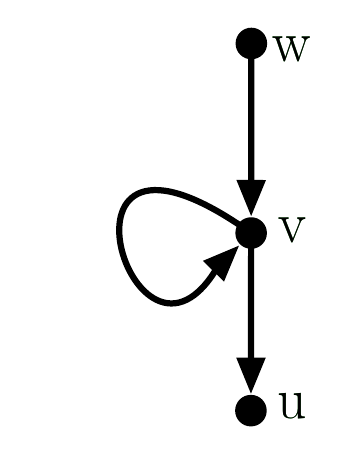
\begin{tikzpicture}[x=0.75pt,y=0.75pt,yscale=-1,xscale=1, opacity=1, fill opacity=1]
%uncomment if require: \path (0,300); %set diagram left start at 0, and has height of 300


%Straight Lines [id:da4670850942943552] 
\draw [line width=2.25]    (231.25,52.67) -- (231.16,126.71) ;
%Curve Lines [id:da34427195808621325] 
\draw [line width=2.25]    (231.14,144) .. controls (124.98,68.18) and (174.97,230.32) .. (215.38,159.61) ;
%Straight Lines [id:da7340515842576736] 
\draw [line width=2.25]    (231.15,138.24) -- (231.06,212.28) ;



%Shape: Triangle [id:dp5511387235098089] 
\draw  [color={rgb, 255:red, 0; green, 0; blue, 0 }][fill={rgb, 255:red, 0; green, 0; blue, 0 }] (231.05,220.06) -- (224.68,204.5) -- (237.45,204.51) -- cycle ;
%Shape: Triangle [id:dp72110595964638] 
\draw  [color={rgb, 255:red, 0; green, 0; blue, 0 }][fill={rgb, 255:red, 0; green, 0; blue, 0 }] (224.33,151.03) -- (217.88,166.55) -- (208.83,157.55) -- cycle ;
%Shape: Triangle [id:dp1921776052623907] 
\draw  [color={rgb, 255:red, 0; green, 0; blue, 0 }][fill={rgb, 255:red, 0; green, 0; blue, 0 }] (231.15,134.49) -- (224.79,118.93) -- (237.55,118.95) -- cycle ;

%Shape: Ellipse [id:dp7930732829426068] 
\draw  [fill={rgb, 255:red, 0; green, 0; blue, 0 }] (231.04,222.47) .. controls (234.97,222.47) and (238.14,225.66) .. (238.14,229.58) .. controls (238.13,233.5) and (234.95,236.68) .. (231.03,236.67) .. controls (227.1,236.67) and (223.93,233.48) .. (223.93,229.56) .. controls (223.94,225.64) and (227.12,222.46) .. (231.04,222.47) -- cycle ;
%Shape: Ellipse [id:dp06243918702040174] 
\draw  [fill={rgb, 255:red, 0; green, 0; blue, 0 }] (231.26,45.57) .. controls (235.18,45.57) and (238.36,48.76) .. (238.35,52.68) .. controls (238.35,56.6) and (235.17,59.78) .. (231.24,59.78) .. controls (227.32,59.77) and (224.14,56.59) .. (224.15,52.66) .. controls (224.15,48.74) and (227.34,45.56) .. (231.26,45.57) -- cycle ;
%Shape: Ellipse [id:dp44126371965490274] 
\draw  [fill={rgb, 255:red, 0; green, 0; blue, 0 }] (231.15,136.9) .. controls (235.07,136.9) and (238.25,140.09) .. (238.24,144.01) .. controls (238.24,147.93) and (235.05,151.11) .. (231.13,151.1) .. controls (227.21,151.1) and (224.03,147.92) .. (224.04,143.99) .. controls (224.04,140.07) and (227.22,136.89) .. (231.15,136.9) -- cycle ;


% Text Node
\onslide<3->{\draw (250.89,55.47) node  [align=left, opacity = 1, ForestGreen] {\huge \poss{w}};
% Text Node
\draw (250.89,142.47) node  [align=left, opacity = 1, ForestGreen] {\huge \poss{v}};
% Text Node
\draw (250.89,227.47) node  [align=left, opacity = 1, ForestGreen] {\huge \poss{u}};
}

% Text Node
\onslide<4->{\draw (250.89,55.47) node  [align=left] {\huge \poss{w}};
% Text Node
\draw (250.89,142.47) node  [align=left] {\huge \poss{v}};
% Text Node
\draw (250.89,227.47) node  [align=left] {\huge \poss{u}};
}

\end{tikzpicture}}}
					\end{center}
				\end{column}}%
			\hfill%
			\onslide<4->{\begin{column}{.35\textwidth}
					{\only<5>{\color{ForestGreen}}
						{\rule{\linewidth}{1pt}
							\footnotesize Relative Kripke Structure}
						\begin{center}
							{\scalebox{0.6}{

\tikzset{every picture/.style={line width=0.75pt}} %set default line width to 0.75pt        

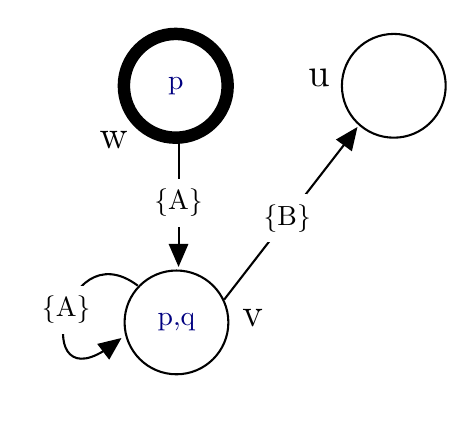
\begin{tikzpicture}[x=0.75pt,y=0.75pt,yscale=-1,xscale=1]
%uncomment if require: \path (0,300); %set diagram left start at 0, and has height of 300

%Straight Lines [id:da7382395640533164] 
\draw    (130.29,59) -- (130.29,118) ;
%Straight Lines [id:da018251469869151382] 
\draw    (152.29,135) -- (213,56.6) ;


%Shape: Circle [id:dp8938158972072578] 
\draw  [line width=0.75]  (104.29,146) .. controls (104.29,132.19) and (115.48,121) .. (129.29,121) .. controls (143.09,121) and (154.29,132.19) .. (154.29,146) .. controls (154.29,159.81) and (143.09,171) .. (129.29,171) .. controls (115.48,171) and (104.29,159.81) .. (104.29,146) -- cycle ;
%Shape: Circle [id:dp19780391712041556] 
\draw   (209,32) .. controls (209,18.19) and (220.19,7) .. (234,7) .. controls (247.81,7) and (259,18.19) .. (259,32) .. controls (259,45.81) and (247.81,57) .. (234,57) .. controls (220.19,57) and (209,45.81) .. (209,32) -- cycle ;
%Shape: Circle [id:dp06782137726568571] 
\draw  [line width=4.5]  (103.95,32) .. controls (103.95,18.19) and (115.15,7) .. (128.95,7) .. controls (142.76,7) and (153.95,18.19) .. (153.95,32) .. controls (153.95,45.81) and (142.76,57) .. (128.95,57) .. controls (115.15,57) and (103.95,45.81) .. (103.95,32) -- cycle ;
%Curve Lines [id:da0862450190271058] 
\draw    (110.62,128.27) .. controls (73.82,100.67) and (58.1,187.08) .. (98.1,157.08) ;

%Shape: Triangle [id:dp4725710951486233] 
\draw  [fill={rgb, 255:red, 0; green, 0; blue, 0 }  ,fill opacity=1 ] (101.8,154.28) -- (96.82,163.08) -- (91.97,156.67) -- cycle ;
%Shape: Triangle [id:dp08394946096129607] 
\draw  [fill={rgb, 255:red, 0; green, 0; blue, 0 }  ,fill opacity=1 ] (215.75,52.87) -- (213.48,62.72) -- (207.01,57.95) -- cycle ;

%Shape: Triangle [id:dp417855807516911] 
\draw  [fill={rgb, 255:red, 0; green, 0; blue, 0 }  ,fill opacity=1 ] (130.29,118) -- (126.27,108.72) -- (134.3,108.72) -- cycle ;


% Text Node
\draw (129.29,146) node  [align=left, NavyBlue] {p,q};
% Text Node
\draw (128.95,32) node  [align=left, NavyBlue] {p};
% Text Node
\draw  [color={rgb, 255:red, 255; green, 255; blue, 255 }  ,draw opacity=1 ][fill={rgb, 255:red, 255; green, 255; blue, 255 }  ,fill opacity=1 ]  (173.64,84.8) -- (191.64,84.8) -- (191.64,106.8) -- (173.64,106.8) -- cycle  ;
\draw (182.64,95.8) node  [align=left] {\{\agentSlide{B}\}};
% Text Node
\draw  [color={rgb, 255:red, 255; green, 255; blue, 255 }  ,draw opacity=1 ][fill={rgb, 255:red, 255; green, 255; blue, 255 }  ,fill opacity=1 ]  (67.14,129) -- (85.14,129) -- (85.14,151) -- (67.14,151) -- cycle  ;
\draw (76.14,140) node  [align=left] {\{\agentSlide{A}\}};
% Text Node
\draw  [color={rgb, 255:red, 255; green, 255; blue, 255 }  ,draw opacity=1 ][fill={rgb, 255:red, 255; green, 255; blue, 255 }  ,fill opacity=1 ]  (121.29,77.5) -- (139.29,77.5) -- (139.29,99.5) -- (121.29,99.5) -- cycle  ;
\draw (130.29,88.5) node  [align=left] {\{\agentSlide{A}\}};
% Text Node
\draw (99,58) node  [align=left] {\Large \poss{w}};
% Text Node
\draw (166,144) node  [align=left] {\Large \poss{v}};
% Text Node
\draw (198,28) node  [align=left] {\Large \poss{u}};


\end{tikzpicture}
}}
						\end{center}
					}
				\end{column}}%
		\end{columns}

		\begin{tikzpicture}[overlay, remember picture]
			\only<2>{\draw[thick, -Stealth,out=180,in=180,looseness=2, ForestGreen] ($({pic cs:froma})+(-1.5ex,0.5ex)$) to ($({pic cs:fromb})+(-1ex,1.1ex)$);}
			\onslide<3->{\draw[thick, -Stealth,out=180,in=180,looseness=2] ($({pic cs:froma})+(-1.5ex,0.5ex)$) to ($({pic cs:fromb})+(-1ex,1.1ex)$);}
			\only<3>{\draw[thick, -Stealth,out=180,in=180,looseness=2, ForestGreen] ($({pic cs:fromb})+(-1.5ex,0.5ex)$) to ($({pic cs:fromc})+(-1ex,1.1ex)$);}
			\onslide<4->{\draw[thick, -Stealth,out=180,in=180,looseness=2] ($({pic cs:fromb})+(-1.5ex,0.5ex)$) to ($({pic cs:fromc})+(-1ex,1.1ex)$);}
			\only<4>{\draw[thick, -Stealth,out=180,in=180,looseness=2, ForestGreen] ($({pic cs:fromc})+(-1.5ex,0.5ex)$) to ($({pic cs:fromd})+(-1ex,1.1ex)$);}
			\onslide<5->{\draw[thick, -Stealth,out=180,in=180,looseness=2] ($({pic cs:fromc})+(-1.5ex,0.5ex)$) to ($({pic cs:fromd})+(-1ex,1.1ex)$);
				\draw[thick, Stealth-Stealth,out=0,in=0,looseness=2, ForestGreen] ($({pic cs:frome})+(1.5ex,0.5ex)$) to ($({pic cs:fromf})+(1ex,1.1ex)$);
				\draw[ForestGreen,thick,rounded corners] ($({pic cs:fromh})+(-0.5ex,-0.7ex)$) rectangle ($({pic cs:frome})+(0.5ex,2ex)$);
				\draw[ForestGreen,thick,rounded corners] ($({pic cs:fromg})+(-0.5ex,-0.7ex)$) rectangle ($({pic cs:fromf})+(0.5ex,2ex)$);}
		\end{tikzpicture}
	\end{frame}
}